% Standalone TikZ figure: shared global/local multi-view retrieval encoder + supervised
% geographic contrastive refinement (T4.1c, CURRENT BEST MODEL, fold-0 screen 150.79km,
% 2026-08-20). Builds on T4.1 (figures/architecture_t4_1.tex, if present) and T4.1b's
% shared-backbone multi-view fusion -- kept as separate files per this project's convention
% of not overwriting earlier architecture figures (see architecture_t3_4.tex's header note).
%
% Compile alone:      tectonic architecture_t4_1c.tex   (or pdflatex/lualatex/xelatex)
%
% All dimensions/params below are the real, verified numbers (src/protocol/param_check.py,
% EfficientNet-B0 RA4 backbone, fold 0):
%   backbone feature dim = 1280, embedding dim = 256, K = 3 independent partitions
%   (96 cells/partition, 8/country x 12 countries), N_COUNTRIES = 12,
%   total params = 4,722,346 (of the 5,000,000 budget, 277,654 unused).
%
% What T4.1c IS, precisely -- a two-stage recipe, not a new architecture class:
%   Stage 1 (T4.1b): train the shared-backbone multi-view retrieval model from an
%     ImageNet-pretrained EfficientNet-B0 RA4 init, 60 epochs, backbone_lr=1e-4/head_lr=1e-3,
%     no contrastive term (contrastive_weight=0). This is the box structure below.
%   Stage 2 (T4.1c, this figure's headline number): CONTINUE from stage 1's best checkpoint
%     for 20 more epochs at 5x lower LR (backbone 2e-5, head 2e-4), now with the supervised
%     geographic contrastive loss switched on (contrastive_weight=0.2, temperature=0.1).
%     Zero new parameters -- same 4,722,346-param network, just further-refined weights.
%     fold0: T4.1b best_model.pt -> 20ep continuation -> 150.79km (best decoder
%     mode_w4_l0_r150, i.e. retrieval_weight=4, local_weight=0, mode radius=150km).
%
% The diagram below shows ONE forward pass (shared for both stages) plus the FULL loss set
% (some active only in stage 2) and the retrieval-based inference decode path.

\documentclass[tikz,border=4pt]{standalone}
\usepackage{amsmath}
\usetikzlibrary{positioning, arrows.meta, fit, backgrounds, shapes.geometric, calc}

\begin{document}
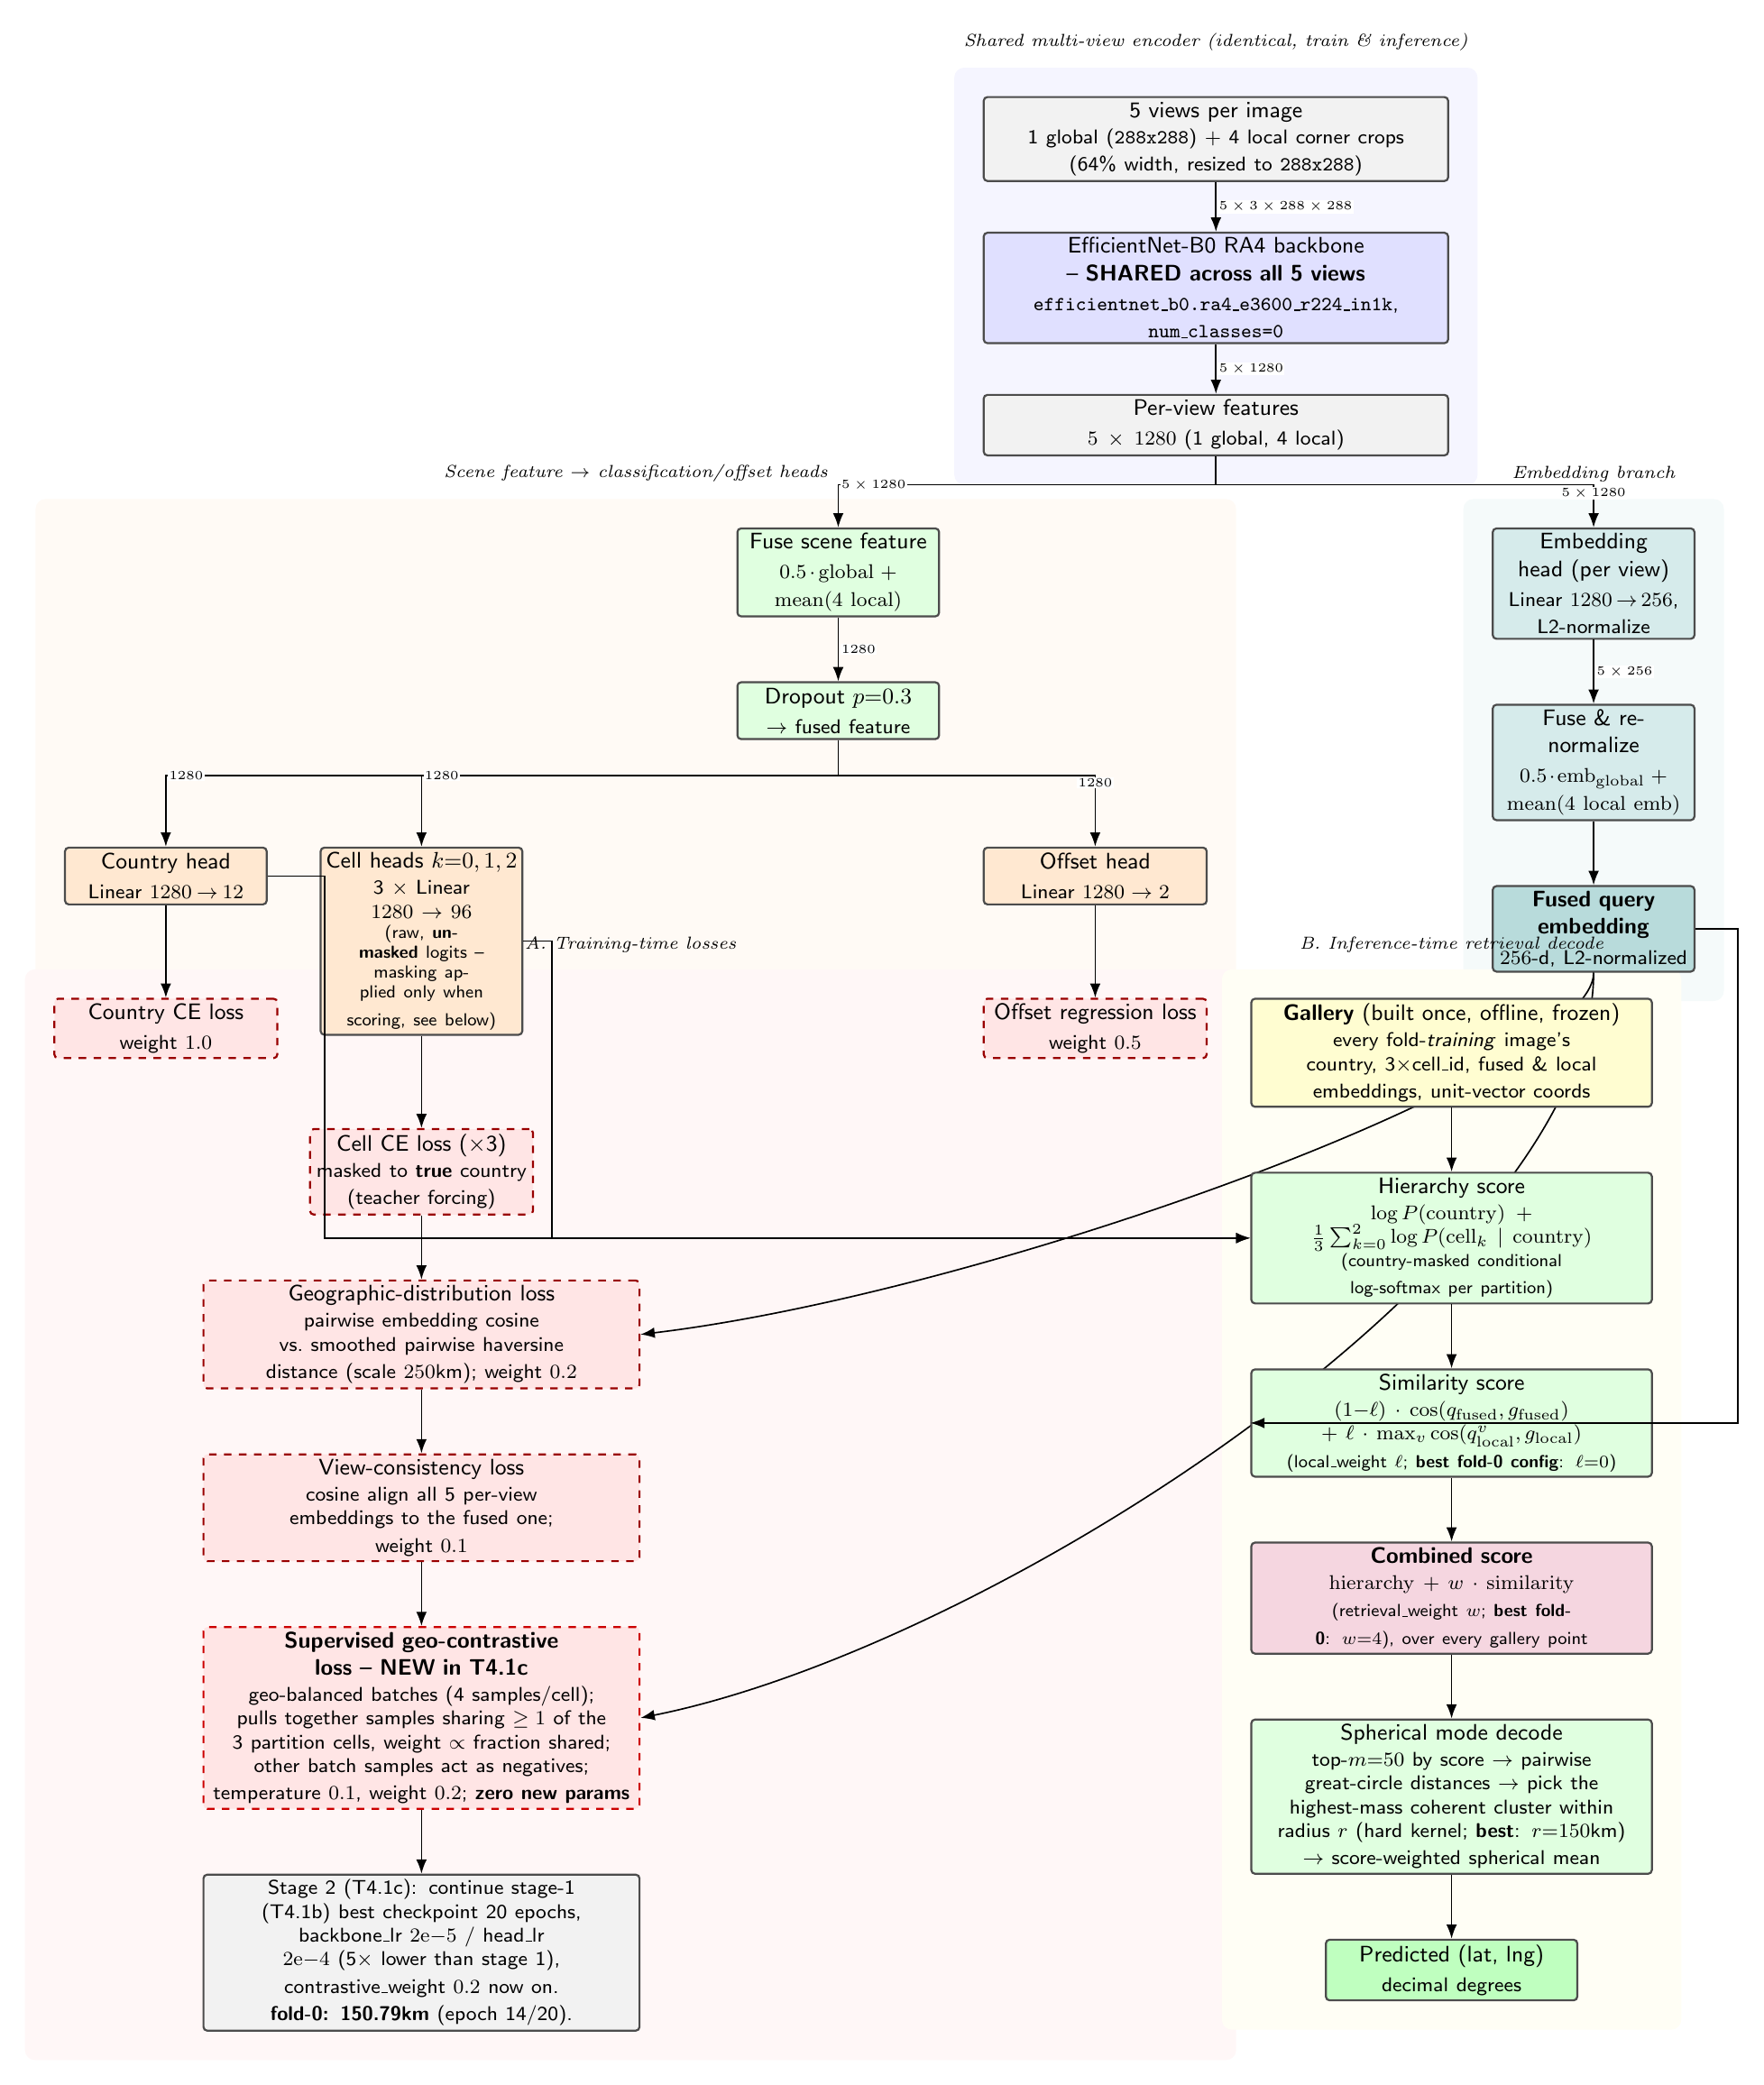
\begin{tikzpicture}[
  font=\sffamily\small,
  node distance=7mm and 9mm,
  >={Latex[length=2mm,width=1.5mm]},
  every path/.style={line width=0.6pt},
  block/.style={
    rectangle, rounded corners=1.5pt, draw=black!70, thick,
    minimum height=8mm, text width=30mm, align=center, inner sep=2pt
  },
  backbone/.style={block, fill=blue!12, text width=64mm},
  head/.style={block, fill=orange!18, text width=27mm},
  emb/.style={block, fill=teal!16, text width=27mm},
  fixed/.style={block, fill=black!8, dashed, text width=27mm},
  op/.style={block, fill=green!12, text width=27mm},
  fuse/.style={block, fill=purple!16, thick, text width=40mm},
  loss/.style={block, fill=red!10, dashed, draw=red!60!black, text width=30mm},
  gallery/.style={block, fill=yellow!18, text width=32mm},
  outnode/.style={block, fill=green!25, thick, text width=34mm},
  dimlabel/.style={font=\tiny\itshape, pos=0.5, right=0.5pt, fill=white, inner sep=0.5pt},
  dimlabelb/.style={font=\tiny\itshape, pos=0.5, below=0.5pt, fill=white, inner sep=0.5pt},
]

% =========================================================================================
% SHARED ENCODER (identical at train and inference time)
% =========================================================================================
\node[block, fill=black!5, text width=64mm] (input)
  {5 views per image\\[1pt]\footnotesize 1 global (\texttt{288x288}) $+$ 4 local corner crops\\
   (64\% width, resized to \texttt{288x288})};
\node[backbone, below=of input] (backbone)
  {EfficientNet-B0 RA4 backbone -- \textbf{SHARED across all 5 views}\\[1pt]
   \footnotesize\texttt{efficientnet\_b0.ra4\_e3600\_r224\_in1k}, \texttt{num\_classes=0}};
\draw[->] (input) -- (backbone) node[dimlabel]{$5\times3\times288\times288$};

\node[block, fill=black!5, below=of backbone, text width=64mm] (perview)
  {Per-view features\\[1pt]\footnotesize $5 \times 1280$ (1 global, 4 local)};
\draw[->] (backbone) -- (perview) node[dimlabel]{$5\times1280$};

% ---- split: scene-feature path (left) vs. embedding path (right) ----
\node[op, below left=10mm and 6mm of perview] (fuse_feat)
  {Fuse scene feature\\[1pt]\footnotesize $0.5\!\cdot\!\mathrm{global} + \mathrm{mean}(4\ \mathrm{local})$};
\node[emb, below right=10mm and 6mm of perview] (emb_head)
  {Embedding head (per view)\\[1pt]\footnotesize Linear $1280\!\to\!256$, L2-normalize};

\draw[->] (perview.south) -- ++(0,-4mm) -| (fuse_feat.north) node[pos=0.3,dimlabel]{$5\times1280$};
\draw[->] (perview.south) -- ++(0,-4mm) -| (emb_head.north) node[pos=0.7,dimlabelb]{$5\times1280$};

\node[op, below=9mm of fuse_feat] (dropout)
  {Dropout $p{=}0.3$\\[1pt]\footnotesize $\to$ fused feature};
\draw[->] (fuse_feat) -- (dropout) node[dimlabel]{$1280$};

\node[emb, below=9mm of emb_head] (fuse_emb)
  {Fuse \& re-normalize\\[1pt]\footnotesize $0.5\!\cdot\!\mathrm{emb}_{\mathrm{global}} + \mathrm{mean}(4\ \mathrm{local\ emb})$};
\draw[->] (emb_head) -- (fuse_emb) node[dimlabel]{$5\times256$};

\node[emb, below=9mm of fuse_emb, fill=teal!28, thick] (final_emb)
  {\textbf{Fused query embedding}\\[1pt]\footnotesize $256$-d, L2-normalized};
\draw[->] (fuse_emb) -- (final_emb);

% ---- four heads off the fused 1280-d feature: country, K=3 cell heads (unmasked), offset ----
\node[head, below left=15mm and 66mm of dropout] (country_head)
  {Country head\\[1pt]\footnotesize Linear $1280\!\to\!12$};
\node[head, below left=15mm and 30mm of dropout] (cell_heads)
  {Cell heads $k{=}0,1,2$\\[1pt]\footnotesize 3 $\times$ Linear $1280\!\to\!96$\\ \scriptsize (raw, \textbf{unmasked} logits --\\ masking applied only when\\ scoring, see below)};
\node[head, below right=15mm and 6mm of dropout, text width=30mm] (offset_head)
  {Offset head\\[1pt]\footnotesize Linear $1280\!\to\!2$};

\draw[->] (dropout.south) -- ++(0,-5mm) -| (country_head.north) node[pos=0.25,dimlabel]{$1280$};
\draw[->] (dropout.south) -- ++(0,-5mm) -| (cell_heads.north) node[pos=0.4,dimlabel]{$1280$};
\draw[->] (dropout.south) -- ++(0,-5mm) -| (offset_head.north) node[pos=0.75,dimlabelb]{$1280$};

% =========================================================================================
% A. TRAINING-TIME LOSSES (dashed red boxes; some active only in T4.1c's stage 2)
% =========================================================================================
\node[loss, below=13mm of country_head] (l_country)
  {Country CE loss\\[1pt]\footnotesize weight $1.0$};
\draw[->] (country_head) -- (l_country);

\node[loss, below=13mm of cell_heads] (l_cell)
  {Cell CE loss ($\times$3)\\[1pt]\footnotesize masked to \textbf{true} country\\ (teacher forcing)};
\draw[->] (cell_heads) -- (l_cell);

\node[loss, below=13mm of offset_head] (l_offset)
  {Offset regression loss\\[1pt]\footnotesize weight $0.5$};
\draw[->] (offset_head) -- (l_offset);

\node[loss, below=9mm of l_cell, text width=60mm] (l_geo)
  {Geographic-distribution loss\\[1pt]\footnotesize pairwise embedding cosine\\ vs.\ smoothed pairwise haversine\\ distance (scale $250$km); weight $0.2$};
\draw[->] (final_emb.south) .. controls +(0,-14mm) and +(50mm,6mm) .. (l_geo.east);
\draw[->] (l_cell) -- (l_geo);

\node[loss, below=9mm of l_geo, text width=60mm] (l_consist)
  {View-consistency loss\\[1pt]\footnotesize cosine align all 5 per-view\\ embeddings to the fused one;\\ weight $0.1$};
\draw[->] (l_geo) -- (l_consist);

\node[loss, below=9mm of l_consist, thick, draw=red!80!black, text width=60mm] (l_contrastive)
  {\textbf{Supervised geo-contrastive loss -- NEW in T4.1c}\\[1pt]
   \footnotesize geo-balanced batches (4 samples/cell);\\
   pulls together samples sharing $\ge\!1$ of the\\
   3 partition cells, weight $\propto$ fraction shared;\\
   other batch samples act as negatives;\\
   temperature $0.1$, weight $0.2$; \textbf{zero new params}};
\draw[->] (l_consist) -- (l_contrastive);
\draw[->] (final_emb.south) .. controls +(0,-40mm) and +(50mm,10mm) .. (l_contrastive.east);

\node[block, fill=black!5, below=9mm of l_contrastive, text width=60mm] (stage2note)
  {\footnotesize Stage 2 (T4.1c): continue stage-1 (T4.1b) best checkpoint 20 epochs,\\
   backbone\_lr $2\mathrm{e}{-5}$ / head\_lr $2\mathrm{e}{-4}$ (5$\times$ lower than stage 1),\\
   contrastive\_weight $0.2$ now on. \textbf{fold-0: 150.79km} (epoch 14/20).};
\draw[->] (l_contrastive) -- (stage2note);

% =========================================================================================
% B. INFERENCE-TIME RETRIEVAL DECODE (right side, from the fused embedding + head logits)
% =========================================================================================
\node[gallery, below right=13mm and 6mm of offset_head, text width=55mm] (gallery_build)
  {\textbf{Gallery} (built once, offline, frozen)\\[1pt]\footnotesize every fold-\emph{training} image's\\
   country, 3$\times$cell\_id, fused \& local\\ embeddings, unit-vector coords};

\node[op, below=9mm of gallery_build, text width=55mm] (hierarchy_score)
  {Hierarchy score\\[1pt]\footnotesize $\log P(\mathrm{country}) + \tfrac{1}{3}\sum_{k=0}^{2}\log P(\mathrm{cell}_k\!\mid\!\mathrm{country})$\\
   \scriptsize (country-masked conditional\\ log-softmax per partition)};
\draw[->] (country_head.east) -- ++(8mm,0) |- (hierarchy_score.west);
\draw[->] (cell_heads.east) -- ++(4mm,0) |- (hierarchy_score.west);
\draw[->] (gallery_build) -- (hierarchy_score);

\node[op, below=9mm of hierarchy_score, text width=55mm] (sim_score)
  {Similarity score\\[1pt]\footnotesize $(1{-}\ell)\cdot\cos(q_{\mathrm{fused}}, g_{\mathrm{fused}})$\\
   $+\ \ell\cdot\max_v \cos(q^v_{\mathrm{local}}, g_{\mathrm{local}})$\\
   \scriptsize (local\_weight $\ell$; \textbf{best fold-0 config}: $\ell{=}0$)};
\draw[->] (final_emb.east) -- ++(6mm,0) |- (sim_score.west);
\draw[->] (hierarchy_score) -- (sim_score);

\node[fuse, below=9mm of sim_score, text width=55mm] (combined_score)
  {\textbf{Combined score}\\[1pt]\footnotesize $\mathrm{hierarchy} + w\cdot\mathrm{similarity}$\\
   \scriptsize (retrieval\_weight $w$; \textbf{best fold-0}: $w{=}4$), over every gallery point};
\draw[->] (sim_score) -- (combined_score);

\node[op, below=9mm of combined_score, text width=55mm] (mode_decode)
  {Spherical mode decode\\[1pt]\footnotesize top-$m{=}50$ by score $\to$ pairwise\\
   great-circle distances $\to$ pick the\\
   highest-mass coherent cluster within\\
   radius $r$ (hard kernel; \textbf{best}: $r{=}150$km)\\
   $\to$ score-weighted spherical mean};
\draw[->] (combined_score) -- (mode_decode);

\node[outnode, below=9mm of mode_decode] (final)
  {Predicted (lat, lng)\\[1pt]\footnotesize decimal degrees};
\draw[->] (mode_decode) -- (final);

% ---- background grouping boxes ----
% NOTE: group labels are added as plain foreground nodes anchored off each fit box's
% `.north`, not via `fit`'s `label=` key -- `label=` on a node placed `on background
% layer` was observed to compute the picture's overall bounding box BEFORE the label
% text's extent, clipping long labels (e.g. "B. Inference-time retrieval decode") at
% the standalone page's right edge. Plain nodes in the normal (foreground) layer are
% always included in the bounding box, so this is used uniformly for all five labels.
\begin{scope}[on background layer]
  \node[fit=(input)(backbone)(perview), fill=blue!4, rounded corners=4pt, inner sep=4mm] (fit_encoder) {};
  \node[fit=(fuse_feat)(dropout)(country_head)(cell_heads)(offset_head), fill=orange!4, rounded corners=4pt, inner sep=4mm] (fit_heads) {};
  \node[fit=(emb_head)(fuse_emb)(final_emb), fill=teal!4, rounded corners=4pt, inner sep=4mm] (fit_emb) {};
  \node[fit=(l_country)(l_cell)(l_offset)(l_geo)(l_consist)(l_contrastive)(stage2note), fill=red!3, rounded corners=4pt, inner sep=4mm] (fit_losses) {};
  \node[fit=(gallery_build)(hierarchy_score)(sim_score)(combined_score)(mode_decode)(final), fill=yellow!4, rounded corners=4pt, inner sep=4mm] (fit_decode) {};
\end{scope}

\node[font=\scriptsize\itshape, above=1mm of fit_encoder.north] {Shared multi-view encoder (identical, train \& inference)};
\node[font=\scriptsize\itshape, above=1mm of fit_heads.north] {Scene feature $\to$ classification/offset heads};
\node[font=\scriptsize\itshape, above=1mm of fit_emb.north] {Embedding branch};
\node[font=\scriptsize\itshape, above=1mm of fit_losses.north] {A. Training-time losses};
\node[font=\scriptsize\itshape, above=1mm of fit_decode.north] {B. Inference-time retrieval decode};

\end{tikzpicture}
\end{document}

% ---------------------------------------------------------------------------------------
% Params (verified via src/protocol/param_check.py, EfficientNet-B0 RA4 backbone):
%   backbone (efficientnet_b0.ra4_e3600_r224_in1k, shared across all 5 views)   4,007,548
%   country head (1280->12)                                                       15,372
%   cell heads k=0,1,2 (1280->96 each, x3)                                       368,928
%   offset head (1280->2)                                                          2,562
%   embedding head (1280->256, shared across all 5 views)                       327,936
%   TOTAL                                                                      4,722,346   / 5,000,000 budget
%
% fold-0 screen results (2026-08-20):
%   T4.1  (single global view, no local crops):            166.85km trained / 160.42km w/ mode decoder
%   T4.1b (this shared multi-view encoder, stage 1 only):  155.07km (job 4063141, epoch 51/60)
%   T4.1c (stage 1 + stage-2 geo-contrastive continuation): 150.79km (job 4065137, epoch 14/20)
%     -- best decoder mode_w4_l0_r150; country acc 77.76%, cell acc (avg/partition) 43.51%.
%   Full 5-fold CV for T4.1c (2026-08-20, jobs 4067429-4067443, stage-1 folds 1-4 chained
%   via SLURM --dependency=afterok into stage-2 folds 0-4): 149.5 +/- 4.6km median
%   (per-fold: 153.45 / 151.79 / 144.44 / 144.56 / 153.28km), mean 449.5km, cell acc 43.7%,
%   country acc 77.0%. NEW BEST result, beating T3.4's 182.9 +/- 7.0km by 33.4km -- tight
%   cross-fold std (4.6km) confirms a real, general improvement. Gap to the ~114-120km
%   reference target narrowed from 68.9km (T3.4) to ~29.5-35.5km. Caveat: folds 1 and 4
%   peaked at continuation epoch 1 and 3 of 20, so most of the gain comes from turning the
%   contrastive loss on at all, not from training it long.
% ---------------------------------------------------------------------------------------
